\documentclass{article}

\usepackage{graphicx}

\title{Effect Network - Decentralised network for Artificial Intelligence \\ \vspace{16pt} \large \textbf{DRAFT}}
\date{\today}
\author{Jesse Eisses, Laurens Verspeek \\
  \small \texttt{\{jeisses, lverspeek\}@effect.ai}}

\begin{document}

\maketitle

\begin{abstract}
Decentralized open network for AI
\end{abstract}

\tableofcontents


\section{Introduction}
In the past half-decade there has been a rapid growth in the number of
practical Artificial Intelligence (AI) applications around us. Smart
services, like self-driving cars, face and voice recognition in mobile
phones and image translation are getting a central place in everyday
life. This rise can be explained by the advances in machine learning
research and the ready availability of cloud computing. This has
resulted in large adoption by the industry and the birth of a
billion-dollar-economy around smart applications. We propose a
private, decentralized ecosystem called the \emph{Effect Network}. The
network is designed to provide a feature complete alternative to the
services shown in Table~\ref{tab:service_compare}, and operates fully
on smart contracts deployed on a Turing-complete blockchain.

\begin{table}
  \centering
  \begin{tabular}[h]{l|l|l}
    \textbf{Market} & \textbf{Suppliers} & \textbf{Market Cap.} \\ \hline
    Micro tasking & Amazone Mechanical Turk, Fiverr, \dots & \dots \\ 
    AI as a service & Watson, Amazon Rekognition, \dots & \dots \\
    Computational platform & Google Cloud ML, Amazone AI, \dots & \dots 
  \end{tabular}
  \caption{Overview of markets (WIP)}\label{tab:service_compare}
\end{table}

\subsection{Blockchain}
A blockchain is a decentralized data store that can contain arbitrary
logic and processes, without the need for a trusted central
party. Blockchain was first proposed in the Bitcoin whitepaper by
Satoshi Nakamoto, 2009\footnote{reference}. Since then the technology
has found application in many areas, and has had a disruptive
influence in the markets of banking, insurance, real-estate and many
more. Decentralized applications have some unique properties like
transparency and no-ownership. We propose a protocol that
decentralizes the global market in Artificial Intelligence; which
reduces the barrier for entry, stimulates market growth and greatly
reduces usage cost.

\subsection{Artificial Intelligence Market}
The AI market will benefit from decentralization because of the high
degree of interaction between agents. Currently, most intelligent
algorithms are developed behind the closed doors of large
corporations, while academic achievements are available to the
public. The main reasons that make practical AI development
inaccessible for individuals are listed below:

\begin{description}
\item[Data processing] Intelligent applications perform tasks that
  traditionally require human feedback. Such tasks involve processing
  unstructured data and finding patterns that can provide useful
  output. These applications are trained on large datasets with
  annotations. Obtaining an annotated dataset is non-trivial and
  requires a lot of time and money.
  
\item[Diverging tasks] An obstacle when developing a complex
  algorithm is the need to interact with parts of the world outside
  the current domain. For example: a self-driving car learning to steer 
  will also need to identify road signs around the world. This
  situation can best be treated as a knowledge system where the
  classification of the sign is done by an external application. This
  quickly increases the amount of work needed.
  
\item[Computational cost] Developing and training a large AI is a
  computational intensive task, and requires a technical
  infrastructure capable of processing terabytes of data, doing
  batched processing on multiple GPUs and coordinating the
  results.
\end{description}

These 3 points are solved by the \emph{Effect Network}. Like other
decentralized applications, \emph{Effect} directly connects supply and
demand without the need for an intermediary party. This brings many
advantages:

\begin{itemize}
\item \textbf{Accessibility.} By directly linking supply and demand
  through our micro-tasking platform (see Section \ref{sec:phase1})
  the \emph{Effect Network} will make training AI algorithms easier,
  faster and cheaper. This will enable people who don't have access to
  a large dataset or a big network to train their AI algorithm.
\item \textbf{Accuracy.} The \emph{Effect Network} is an exchange with
  a rich ontology of specialist AI applications. Individual
  applications can find each other to buy or sell information, as
  specified in Section \ref{sec:phase2}. Through this exchange users
  can use data sets with significantly higher complexities to train
  their AI algorithms.
\item \textbf{Performance.} People can directly buy existing datasets
  on the \emph{Effect Exchange} (Section \ref{sec:phase2}) or quickly
  create their own dataset by creating micro-task on the \emph{Effect
    Mechanical Turk} platform (Section \ref{sec:phase1}). By enabling
  people to retrieve accurate datasets quickly, they can immediately
  use these datasets to train AI Algorithms.
\item \textbf{Interoperability.} By putting the AI algorithms on the
  blockchain and creating a standard to which these AI algorithms have
  to comply to, we can truly decentralize AI and achieve
  interoperability between individual AIs. The combination of multiple
  AI algorithms will result in powerful capabilities and emergent
  intelligence that no single AI algorithm can achieve on his own.
\end{itemize}

The network will be deployed in consecutive phases, allowing adaption
and development of the network to grow together. The phases cover
independent market section, but are interconnect in our network model,
and are all fueled by the same token, called \emph{AIX}.

\section{Phase 1: Decentralized Mechanical Turk}
\label{sec:phase1}
The \emph{Effect Mechanical Turk} platform is a decentralized, peer to
peer marketplace for work that requires human intelligence.  It
provides similar features as centralized services like Amazon
Mechanical Turk\footnote{https://www.mturk.com}, Fiverr\footnote{},
Crowdsource\footnote{} and Guru.com\footnote{}. It is a crowd sourcing
technology that enables requesters to submit tasks that can be
completed by human agents in exchange for compensation. Users can work
on tasks from requesters at any time, anywhere and from any
device. The tasks are called Human Intelligence Tasks (HIT). The
providers of the HIT’s are called \emph{requesters}. When a user
completes a task, they are paid with with a network token called AIX.

\begin{figure}[htb]
  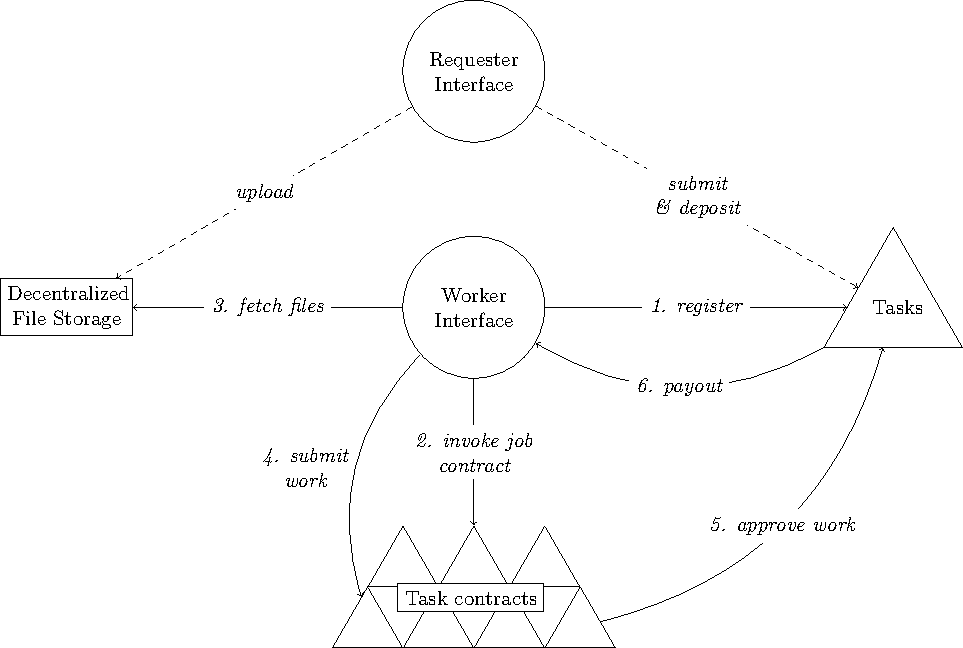
\includegraphics[width=\textwidth]{pictures/emt.pdf}
  \caption{Process of submitting jobs on the \emph{Effect Mechanical Turk}}
\end{figure}


\subsection{Requesters}
\emph{Effect Requesters} can put tasks (see Section
\ref{subsec:tasks}) on the \emph{Effect Mechanical Turk} platform to
be completed by workers. the requestors can decide how many AIX the
workers will get for each completed task. The requestors can retrieve
the results from the \emph{Effect Mechanical Turk} platform and use
these results to, for example, train their AI algorithm. \emph{Effect
  Mechanical Turk} gives requestors access to an on-demand, scalable
and distributed workforce.

\subsection{Workers}
\emph{Effect Workers} can complete the tasks from the requestors in
exchange for the AIX tied to these tasks (see Section
\ref{subsec:tasks}).

\subsection{Tasks}
\label{subsec:tasks}
A task refers to a dataset that can contain any amount of media
assets. The contract ID of the task will validate the format of the
data. Extracting and presenting examples form the dataset is done by
the user interface.

A task has at least the following properties:

\begin{table}[h]
  \centering
  \begin{tabular}[h]{r|l}
    Dataset & URL \\
    Description & description of the task \\ 
    Contract ID & smart contract that will handle task \\
    Blueprint & data for the contract \\ 
    Required \emph{honor} & require trusted users \\
    Reward & rewarded AIX upon completion \\
    Num. ratings & number of ratings per user \\
    Rating timeout & timeout on performing a rating \\ 
    Expiration  & block ID after which task expires \\
    Sequence id & for sequencing examples (optional)\\
    Data credentials & to unlock private datasets \\
  \end{tabular}
  \caption{Properties of a task}
  \label{tab:task}
\end{table}

The structure and required feedback for a task are defined by the
contract ID and the blueprint. Each type op task requires a smart
contract to handle. \emph{Effect} maintains a database of deployed
smart contracts to make it easy for requesters and workers to interact
with the network. Adding smart contracts to the network is handled
through governance (section~\ref{}). Affiliate programs
will cover costs of deploying new contract types. 

\subsection{Data sets}
Data sets are often large and consist of various types of media. A
blockchain is not a suitable database for storing this kind of
information. Other decentralized storage options, like
BitTorrent\footnote{} and IPFS\footnote{}, are specialized in these
types of assets. For this reason the network will use such a
hash-based distributed file storage, where each media asset can be
revered to by a single hash.

Note that the feedback on a \emph{task} can also involve storing media
assets, for example in tasks like image segmentation. In this case the
ratings asset will be stored on the distributed storage, and a hash
and checksum of the rating are stored on the blockchain.

Requesters will also be able to supply datasets through traditional
channels, like Amazone S3, Google Cloud Storage and FTP.

\subsection{Privacy}
The blockchain is decentralized and open by nature. There are several
measures that must be taken to make sure the Effect network can be
used for sensitive information. The network can provide privacy for
the following cases:

\begin{description}
\item[Datasets] Requesters can provide their dataset in encrypted
  form. Only selected users will be able to decrypt or access the
  data. This is determined by network smart contracts using Public Key
  Encryption, where selected users can decrypt the dataset
  credentials.
\item[User ratings] Tasks performed by users are stored with Public
  Key Encryption. 
\end{description}

Tasks that involve privacy features will be more computational
expensive, thus will also have a higher network fee.

\section{Phase 2: Decentralized AI Exchange}
\label{sec:phase2}

The \emph{Effect AI Exchange} is a decentralized marketplace where
algorithms can exchange their services. An application owner can
register on the exchange by specifying a public endpoint of his
application, following our data interchange format and specifying a
usage fee for consumers. This application can now be invoked through
smart contracts on the blockchain. The caller of the contract will
have to transfer the required funds to the owner of the contract to
get an authorization token that allows him to interact with the application.

Thanks to the application registry, algorithms are able to explore
possible collaborations over the blockchain. It also encourages
standardization of data exchange formats, as interoperability with
other applications means more interactions: a financial incentive.

\subsection{Application registry}
The network will maintain a registry of available applications. This
registry will be enriched with a semantic ontology that describes the
application, as well as a technical schema of its the inputs and
outputs.

\subsection{Endpoints}
Application endpoints on the \emph{Effect AI Exchange} communicate
over the HTTP protocol. Data is exchanged in JSON format and should
strongly confirm the defined RDF schema.

Requests signed with the private key of the buyer will be accepted by
the endpoint. Issuing authorization tokens and checking their validity
can be done by public APIs that hold a partial index of the
blockchain. They could request small fees for providing this service.


\section{Phase 3: Decentralized AI Algorithms}
\label{sec:phase3}
- Put AI algorithms on the blockchain. The algorithms can interact with each other\dots -

\section{Community}
The described network can be deployed and used as a decentralized
application as-is. However, in order for the network to grow and be
sustainable, we believe there has to be a form of governance. Parties
should have incentive to use the AIX token for the purpose AI
tasks. Investors looking for quick monetary gain should be discouraged
and pump-and-dump schemes should be avoided, in order for the network
to grow and slowly take market value from the existing centralized
services.

\subsection{AIX and the Galaxy Pool}
It is important to maintain liquidity in AIX, especially during the
early days when there is no listing on exchanges. Ideally the
following actions should always be possible:

\begin{enumerate}
\item Workers are able to sell their AIX rewards for native tokens
\item Requesters and network users should are able to buy AIX
\end{enumerate}

For a new token on the market this kind of liquidity can be hard to
achieve and can be hurt by speculative trading.

The Effect Network will maintain a central pool of tokens to provide
liquidity, encourage adoption and stabilize network fees. This pool is
called the Galaxy Pool and consists of a mix of AIX and native
tokens. Several rules will drive the Galaxy Pool towards an
equilibrium balance. These rules can later be refined by means of
governance as is discussed in section~\ref{sec:governance}.

\begin{figure}[htb]
  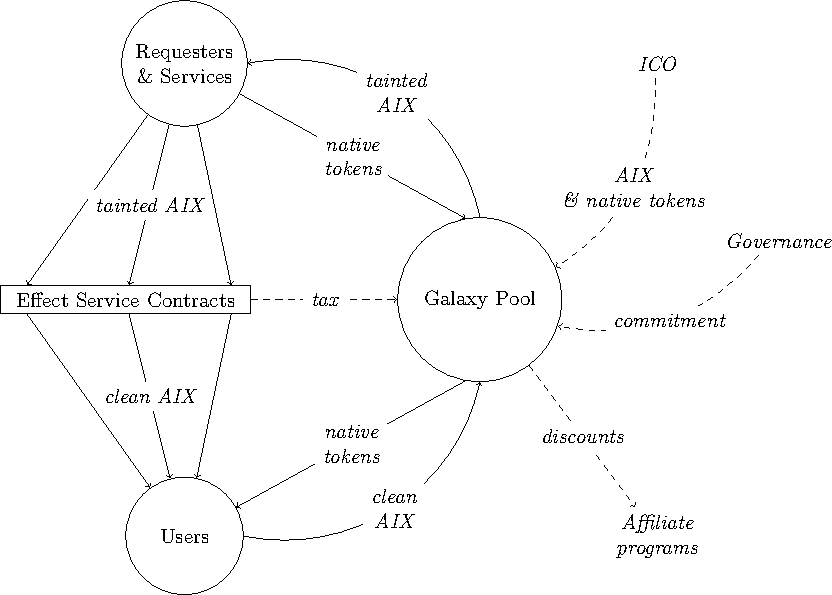
\includegraphics[width=\textwidth]{pictures/galaxy.pdf}
  \caption{Diagram of the \emph{Effect} governance model and
    construction of the Galaxy Pool}
\end{figure}

The Galaxy Pool ensures stable exchange rates for users of the
platform at all times. The pool is not suitable for day traders, as
only \emph{tainted} coins can be bought. Any coin that is bought from
the Galaxy will initially be tainted, and a tainted coin can not be
sold back to the pool. A trainted coin \emph{washed} (converted to a
regular AIX token) by spending it through an \emph{Effect} service
contract. These are the service contracts from the jobs and service
registry. This protects the Galaxy Pool from external manipulation and
keeps exchange rates stable for workers.

\subsection{Honor Tokens and Fraud}
The honor token is a token that can not be traded


\subsection{Proof of Commitment and Governance}
\label{sec:governance}

\section{Examples}

\section{Note on Ethics}

\end{document}